\section{Interaction}
The user interacts with \projectname{} through \deno{B}.
\at{1} and \at{2} dictates the user must be granted access to the system before being able to interact with it.
This access is granted through a valid login and privileges.
When \deno{B} initiates a connection to \deno{M}, \deno{M} returns a login screen as a view.
This is done by the access controller, which is described in Figure~\ref{tab:access_controller_actions} in Appendix~\ref{app:controller_actions}.
The user enters his login credentials in \deno{B} and \deno{B} send a login request to \deno{M}.
The access controller attempts to login the user and if succesfull the user is forwarded the main menu, which is returned as a view from the access controller.
Following a succesfull login the users credentials is stored on \deno{B} as described in Section~\ref{sec:design_client}. \\

\deno{B} can then interact with any of the models described in Section~\ref{section:uml_notation} that have associated views.
The general interaction with these models is similar, and the interaction with drones is described as an example.
When \deno{B} requests to interact with drones, the drone controller returns a view containing a list of all drones available to the user.
This list contains all drones the user has access to based on his privileges.
The users privileges are retrieved through the users model.
For each drone in the system it is checked if the user has privileges that grants him access to the drone.
From the drones list the user can edit a drone, or delete a drone.
Drones are added automically to the system through the initialization messages send by the \deno{Slaves}.
To make a drone usable in \projectname{}, it must be added to a company as reflected in the object model, see Section~\ref{subsec:objects}.
Drones are edited through the edit view returned by the drones controller.
This view is send to \deno{B} from \deno{M} when the user request to edit a drone.

\begin{figure}[htb]
    \centering
    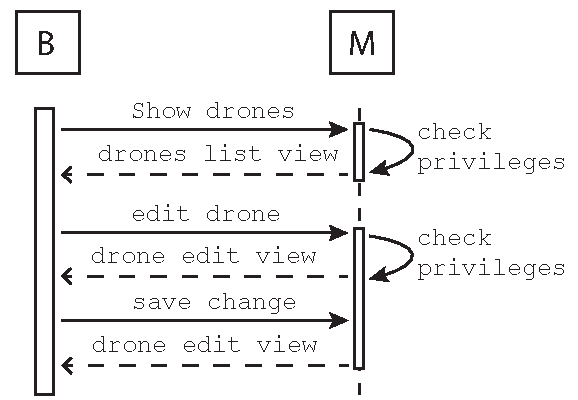
\includegraphics[width=\textwidth]{gfx/interaction_sequence_diagram.pdf}
    \caption{Illustration interaction between \deno{B} and \deno{M}.}
    \label{fig:interaction_sequence}
\end{figure}

\fxfatal{Section om drones list view ellet hvad det nu hedder, skal skrives efter privileges er skrevet}
\fxfatal{User eller \deno{B} n�r vi snakker om brugeren}

From the drones' list \deno{B} can request to pilot or view of the drones' listed.
When \deno{B} requests to pilot a drone the process of retrieving a session key from the drones' associated \deno{S} is initiated by the drones controller.
\deno{B} is redirected to a page containing the video player described in Section~\ref{sec:design_client} when the session key is recieved.
From this page \deno{B} can view the drones video feed and send control commands to the drone as described in Sections~\ref{sec:design_client} and \ref{sec:design_slave}.


%Login -> access i systemet, noget med privileges
%Interaction with 